\documentclass[a4paper,14pt]{extreport}
  \usepackage[left=1.5cm,right=1.5cm,
      top=1.5cm,bottom=2cm,bindingoffset=0cm]{geometry}
  \usepackage{scrextend}
  \usepackage[T1,T2A]{fontenc}
  \usepackage[utf8]{inputenc}
  \usepackage[english,russian,ukrainian]{babel}
  \usepackage{tabularx}
  \linespread{1.3}
  \usepackage[colorinlistoftodos]{todonotes}
  \usepackage{amssymb}
  \usepackage{color}
  \usepackage{amsmath}
  \usepackage{mathrsfs}
  \usepackage{listings}
  \usepackage{graphicx}
  \graphicspath{ {./images/} }
  \usepackage{lipsum}
  \usepackage{xcolor}
  \usepackage{hyperref}
  \usepackage{tcolorbox}

  \usepackage[framemethod=TikZ]{mdframed}
  \usepackage{wrapfig,boxedminipage,lipsum}
  \mdfdefinestyle{MyFrame}{%
  linecolor=blue,outerlinewidth=2pt,roundcorner=20pt,innertopmargin=\baselineskip,innerbottommargin=\baselineskip,innerrightmargin=20pt,innerleftmargin=20pt,backgroundcolor=gray!50!white}
   \usepackage{csvsimple}
   \usepackage{supertabular}
  \usepackage{pdflscape}
  \usepackage{fancyvrb}
  %\usepackage{comment}
  \usepackage{array,tabularx}
  \usepackage{colortbl}

  \usepackage{varwidth}
  \tcbuselibrary{skins}
  \usepackage{fancybox}
  \usepackage{spreadtab}


  \usepackage{tikz}
  \usepackage[framemethod=TikZ]{mdframed}
  \usepackage{xcolor}
  \usetikzlibrary{calc}
  \makeatletter
  \newlength{\mylength}
  \xdef\CircleFactor{1.1}
  \setlength\mylength{\dimexpr\f@size pt}
  \newsavebox{\mybox}
  \newcommand*\circled[2][draw=blue]{\savebox\mybox{\vbox{\vphantom{WL1/}#1}}\setlength\mylength{\dimexpr\CircleFactor\dimexpr\ht\mybox+\dp\mybox\relax\relax}\tikzset{mystyle/.style={circle,#1,minimum height={\mylength}}}
  \tikz[baseline=(char.base)]
  \node[mystyle] (char) {#2};}
  \makeatother
   % Цвета для гиперссылок
  \definecolor{linkcolor}{rgb}{0, 0.72, 0.92} % цвет ссылок
  \definecolor{urlcolor}{rgb}{0.0, 0.0, 1.0}% цвет гиперссылок
  %\hypersetup{pdfstartview=FitH,  linkcolor=linkcolor,urlcolor=urlcolor,citecolor=red, colorlinks=true}

  \definecolor{ggreen}{rgb}{0.4,1,0}
  \definecolor{rred}{rgb}{1,0.1,0.1}
  \definecolor{amber}{rgb}{1.0, 0.75, 0.0}
  \definecolor{babyblue}{rgb}{0.54, 0.81, 0.94}
  \definecolor{amethyst}{rgb}{0.6, 0.4, 0.8}

  \usepackage{float}
  \usepackage{wrapfig}
  \usepackage{framed}
  %for nice Code{
  \lstdefinestyle{customc}{
    belowcaptionskip=1\baselineskip,
    breaklines=true,
    frame=L,
    xleftmargin=\parindent,
    language=C,
    showstringspaces=false,
    basicstyle=\small\ttfamily,
    keywordstyle=\bfseries\color{green!40!black},
    commentstyle=\itshape\color{purple!40!black},
    identifierstyle=\color{blue},
    stringstyle=\color{orange},
  }
  \lstset{escapechar=@,style=customc}
%}


\begin{document}
\renewcommand{\bibname}{Список використаної літератури}% -- переименуем название списка литературы


%указатель -- \cite{lit1}

\pagecolor{white}

%----------------------------------------1
\newtcbox{\xmybox}[1][red]{on line, arc=7pt,colback=#1!10!white,colframe=#1!50!black, before upper={\rule[-3pt]{0pt}{10pt}},boxrule=1pt, boxsep=0pt,left=6pt,right=6pt,top=2pt,bottom=2pt}

\begin{titlepage}
  \begin{center}
  \large
  Національний технічний університет України \\ "Київський політехнічний інститут імені Ігоря Сікорського"


  Факультет Електроніки

  Кафедра мікроелектроніки
  \vfill

  \textsc{РЕФЕРАТ}\\

  %{\Large Про виконання лабораторної роботи №1\\
  з дисципліни: «Фізико - технологічні основи наноелектроніки-2»\\[1cm]

  Прилади на наноструктурованих п'єзоматеріалах


  %}
  \bigskip
  \end{center}
  \vfill

  \newlength{\ML}
  \settowidth{\ML}{«\underline{\hspace{0.4cm}}» \underline{\hspace{2cm}}}
  \hfill
  \begin{minipage}{1\textwidth}
  Виконавець:\\
  Студент 4-го курсу \hspace{4cm} $\underset{\text{(підпис)}}{\underline{\hspace{0.2\textwidth}}}$  \hspace{1cm}Лищенко Б. В.\\
  \vspace{1cm}

  Перевірив: \hspace{5.6cm} $\underset{\text{(підпис)}}{\underline{\hspace{0.2\textwidth}}}$  \hspace{1cm} Орлов А. Т.\\

  \end{minipage}

  \vfill

  \begin{center}
  2021
  \end{center}
\end{titlepage}
\tableofcontents
\setcounter{page}{2}

\newpage

\chapter{Вступ}\par
  %\section{Подраздел}
Величезна кількість п'єзоелектричних матеріалів було продемонстровано з часу відкриття п'єзоелектрики понад століття тому. Однак використання наноструктурованих п’єзоелектриків є відносно недавнім розвитком, і розуміння впливу нанорозмірного розміру на сегнето- та п’єзоелектрику все ще формується. Незважаючи на це, застосування п’єзоелектричних наноструктур для збору енергії швидко розширилося за останнє десятиліття, що призвело до величезного спектру зареєстрованих пристроїв. Більшість досліджень зосереджені на оксиді цинку, оскільки його наноструктури формуються відносно легко за допомогою низькотемпературних методів, на відміну від багатьох сегнетоелектриків, які вимагають високотемпературної обробки. Крім того, наноструктури кристалографічно вирівняні та не сегнетоелектричні, і тому не потребують полірування. Однак останнім часом інші добре відомі матеріали були досліджені для наноструктурованих накопичувачів енергії, включаючи титанат цирконату свинцю (PZT) і титанат барію, з потенціалом більш високої вихідної потужності через їх більш високі п’єзоелектричні коефіцієнти. У цьому огляді підсумовується робота над наноструктурованими п’єзоелектричними збирачами енергії, які зазвичай називають наногенераторами, починаючи з ранніх повідомлень про п’єзоелектричний вихід з одиничних напружених наностержнів ZnO і переходячи до використання масивів наностержнів, гнучких підкладок та альтернативних матеріалів і наноструктур. Узагальнено приклади, які були продемонстровані для пристроїв, і розглянуті майбутні перспективи цієї галузі.
 
 

%%%%%%%%%%%%%%%%%%%%%%%%%%%%%%%%%%%%%%%%%%%%%%
\chapter{Експериментальні методи}\par 

Наностержень ZnO вирощували на 2$\times$1 см оксиду індію-олова (ITO)-
підкладки з поліетилентерефталату (ПЕТ) з покриттям (Aldrich)
засіяний розпиленим ZnO ( плівкою в 100 нм). Посіяні субстрати
суспендують в розчинах 25 мМ нітрату цинку та 25 мМ
гексаметилентетрамін і розігрівають до 90°С протягом 2,5 годин. Це
процес повторювали загалом 6 разів у свіжих розчинах. ZnO
з наностержнів виготовляли пристрої без подальшої обробки
покриття полі(метилметакрилатом) (PMMA) або полі(3,4-
етилендіокситіофен) полі(стиролсульфонат) (PEDOT:PSS).
Три шари 10\%-ного розчину ПММА (Aldrich, Mw 120 000)
в анізолі (Sigma-Aldrich, 99\%) наносили на нанострижні при 1000 об/хв протягом 30 секунд, сушили протягом 10 хвилин при 100$^{\circ}$C
після кожного шару. Два шари отриманого PEDOT:PSS   були нанесені на нанострижні при 2000 об/хв протягом 30 секунд з десятихвилинним сушінням
при 100$^{\circ}$С після кожного шару. Усі пристрої були закінчені випарюванням
золоті контакти на верхній поверхні PMMA або PEDOT:PSS
за допомогою термічного випаровування 99,99+\% золотого дроту (Goodfellows).
Плоскі мідні стрічки були приклеєні як до шару ITO, так і до золота
контакт за допомогою срібного DAG, а потім епоксидної смоли на одному кінці пристрою
(як показано на рис. 2.1е), який був затиснутий для випробування. Сканування
електронно-мікроскопічні (SEM) мікрофотографії наностержнів ZnO були
записано за допомогою FEI Inspect-F SFEG SEM.\\ 

\begin{figure}[h!]
\center{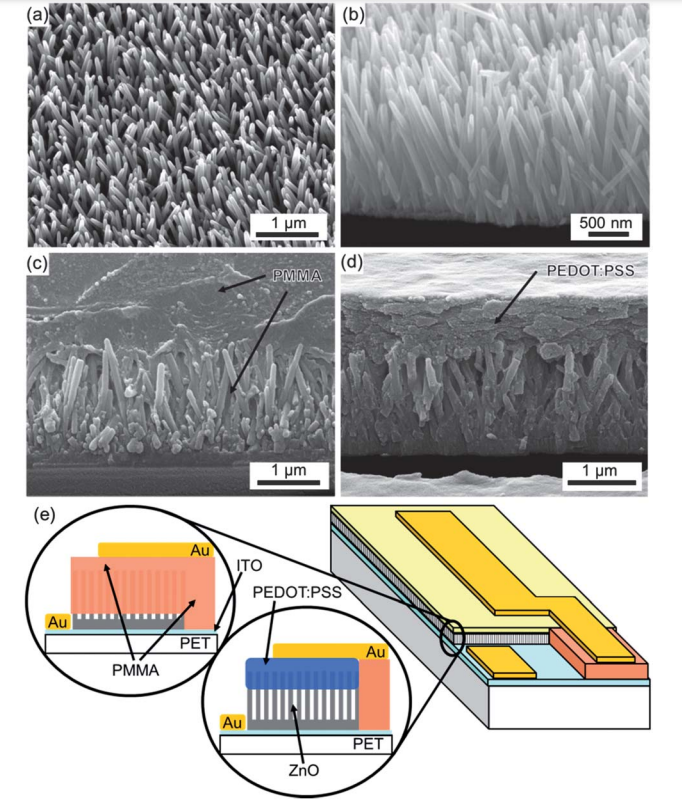
\includegraphics[width=0.9\linewidth]{1b.png}}
\caption{\small{Мікрофотографії та схеми SEM без покриття та з полімерним покриттям ZnO
наностержнів, використаних у дослідженні. (а) 30 нахил наностержнів ZnO без покриття. (b) Перетин наностержнів ZnO. (c) Поперечний переріз наностержнів ZnO, покритих ПММА. PMMA заповнює між наностержнями до основи і покриває їх на 3,5 мм. Верхня частина
шар ПММА обрізається на зображенні, щоб показати деталі заповнення. (d) Поперечний переріз
PEDOT: наностержні ZnO з покриттям PSS. PEDOT:PSS покриває лише кінчики і покриває їх
нанострижні на 1 мм. (e) Схема конструкції пристрою з поперечними перерізами ПММА
та пристрої, що показують різне наповнення, як показано в (c) і (d).}}
\end{figure}

Ефективність збору кінетичної енергії вимірювали за допомогою
монтажу приладів на товщину 0,5 мм, 6 ПЕТ 2,5 см
підкладки та згинання за допомогою кулачка, прикріпленого до двигуна
обертаються з частотою 1–3 Гц так, щоб кінчик підкладки був протилежний контактам
був зігнутий на 10 мм і повертався один раз за цикл. За допомогою камери
можна було підтримувати постійне максимальне зміщення
пристрою, змінюючи частоту деформації. Наведені результати для швидкостей деформації 1 Гц, якщо не вказано інше.
Профіль зміщення руху вимірювали за допомогою MEL
Лазерний тріангуляційний датчик М5. Швидкість обчислювалася з
вимірювання зміщення, що залежать від часу. Напруга, створювана пристроями, була вловлена в розімкненому ланцюзі за допомогою
Осцилограф Tektronix TDS2012C в режимі запуску та з використанням National Instruments NI PXIe-1062Q з підтримкою NI DAQ
в діапазоні навантажень, змінених за допомогою програмованого M-602
десятиліття стійкості (MEATEST). Виправлено опір навантаження
вхідний опір вимірювання 1 MU.
DC-вольтамперні характеристики вимірювали за допомогою
Keithley 2400 SMU в поєднанні з NI Labview. Опір
пристроїв PMMA і PEDOT:PSS вимірювали за допомогою Agilent
4294A Аналізатор імпедансу. Діапазон вхідних частот становив 40
Гц до 10 МГц.


%%%%%%%%%%%%%%%%%%%%%%%%%%%%%%%%%%%%%%%%%%%%%%
\chapter{Електричні характеристики приладів}\par 


Вимірювання електричних властивостей, таких як струм-
Напруга (I–V), ємність–напруга (C–V) та спектроскопія імпедансу можуть дати цінне уявлення про продуктивність пристрою та його зв’язок із структурою та механізмом
перетворення енергії. Такі вимірювання дають корисну інформацію
про внутрішній опір, ємність і випрямлення
поведінку пристроїв.\\ 
\begin{figure}[h!]
\center{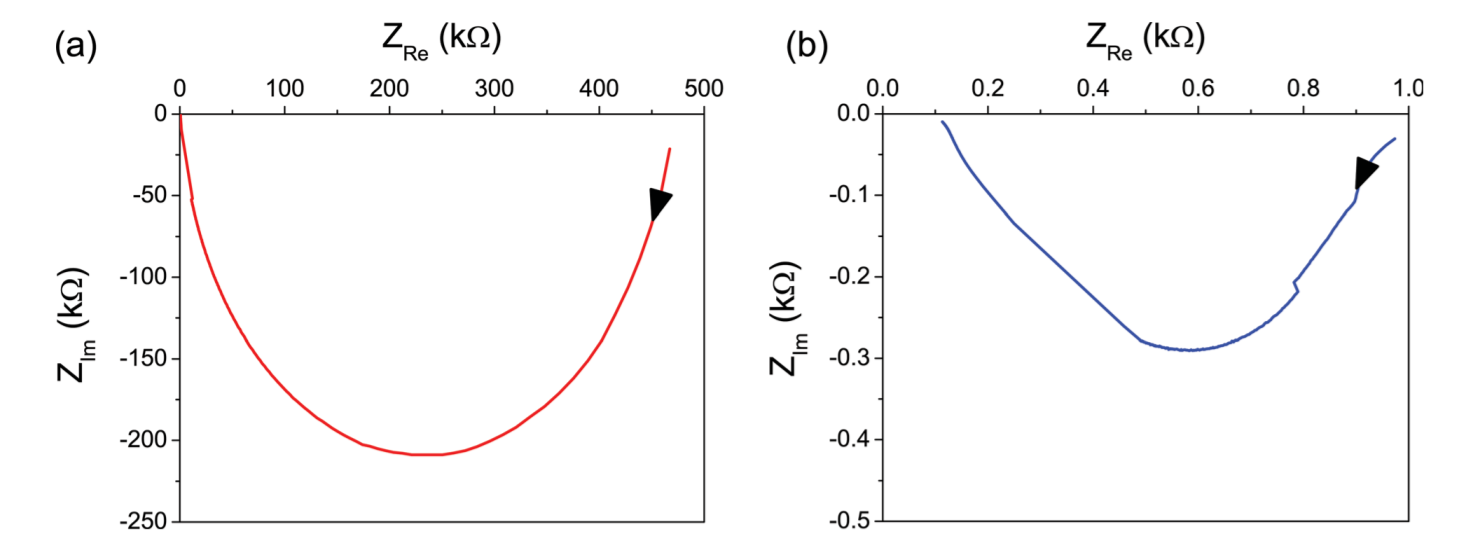
\includegraphics[width=0.9\linewidth]{3b.png}}
\caption{\small{Графіки Найквіста для пристроїв ZnO/PMMA (a) і ZnO/PEDOT:PSS (b), що показують реальні та уявні компоненти імпедансу (Z), виміряні між 40 Гц і
10 МГц. Стрілки позначають напрямок збільшення частоти. Приблизні значення внутрішнього опору та ємності, отримані з аналізу графіків, припускаючи a
Проста RC схема наведена в таблиці 1.)}}
\end{figure}
Поведінка постійного струму-густина-напруга (J–V)
Пристрої ZnO/PMMA та ZnO/PEDOT:PSS показані на рис. 3.1.
Структура ZnO/PMMA (рис. 3.1а) демонструє нелінійну поведінку с
високий опір 1,48 MОм при низькій напрузі і пробою до
набагато нижчого опору близько 530 Ом вище $\pm $1–2 В. ZnO/
PEDOT:PSS поводиться як неідеальний p–n-перехід, тобто
очікується, оскільки вирощений ZnO має n-тип, а PEDOT:PSS – p-тип.  Для ZnO/PEDOT:PSS з використанням неідеального рівняння діода40 з опором послідовно і паралельно (шунт)
діоду, послідовний ($R_{s}$) і шунтовий ($R_{sh}$) опір можна оцінити з поведінки струму навантаження при високому прямому струмі і при зворотному насиченні відповідно. Це дає $R_{s}=$
165 Ом та $R_{sh}$ = 1,55 КОм для діода ZnO/PEDOT:PSS.
Графіки Найквіста, що показують частотно-залежну реактивність
імпеданс ($Z_{Im}$) і частотно-незалежний резистивний опір ($Z_{Re}$) для пристроїв ZnO/PMMA і ZnO/PEDOT:PSS є
показано на рис. 3.2 зі стрілками, що позначають зростання частоти
вимірювання від 40 Гц до 10 МГц. Чисто негативний
уявний імпеданс вказує, що реактивна складова є
ємніснісною. Тому для наближення резистивних і ємнісних властивостей приладів був проведений аналіз
виконується за умови простої RC-схеми.41 У цьому випадку
внутрішній опір можна приблизно визначити з діаметра
кривої вздовж осі, що позначає дійсну складову
імпеданс ($Z_{Re}$), оскільки на низькій частоті імпеданс RC є
суто резистивний. Це дає значення внутрішнього опору ($Z_{int}$).
приблизно 475 КоМ для пристрою PMMA і 1 КоМ для пристрою
Пристрій PEDOT:PSS. Це відповідає вищому опору
значення, отримані із співвідношення струм-напруга для
Пристрій ПММА. Крім того, внутрішній опір для обох
приладів дуже близькі до значень оптимальних опорів навантаження, що очікується, оскільки внутрішній опір
визначає оптимальний опір навантаження.\\ 

Для RC-ланцюга $Z_{Im}$ знаходиться на максимумі на відсіченні або критичній
частоті, $f_c$, що становить 980 Гц для PMMA і 6,7 кГц для
PEDOT:PSS. На цій частоті:
\[ RC = \dfrac{1}{2\cdot \pi f_{c}}\]
З цього можна розрахувати внутрішню ємність,
$C_{int}$, що становить 0,32 нФ для пристрою PMMA і 24 нФ для
PEDOT:PSS. Це наближення, ймовірно, буде більш точним
для пристрою PMMA, оскільки він більше слідує поведінці RC
де ємнісний реактивний опір $X_{c}$ = $R_{int}$/2 при $f_c$, тоді як для
PEDOT:PSS Xc ближче до $R_{int}$/4 у $f_c$. Хоча це тільки
приблизні значення, нижня ємність для пристрою PMMA
буде забезпечувати менше потужності реактивному навантаженню, оскільки це пропорційно ємності. Ці графіки імпедансу можуть забезпечити
набагато важливішу інформацію про деякі складності
електричних характеристик цих пристроїв через більше
поглиблений аналіз і налагодження більш складних схем моделі.
Це триває і має на меті забезпечити повне розуміння
принципів роботи приладів. \\ 

\begin{figure}[h!]
\center{\includegraphics[width=0.9\linewidth]{2и.png}}
\caption{\small{Характеристики густини струму та напруги пристроїв ZnO/PMMA (а) та ZnO/PEDOT:PSS (б)}}
\end{figure}

Цей аналіз демонструє, що розуміння
Вихід, що залежить від навантаження, можна отримати в порівнянні з
електричні властивості самих приладів. Це демонструє
що високий внутрішній резистивний опір пристрою PMMA
призводить до того, що він відповідає очікуваному високому опору навантаження, і
тому дає низьку вихідну потужність порівняно з
пристроями PEDOT:PSS, незважаючи на дещо вищу напругу розімкнутого ланцюга.
Різна ємність двох пристроїв також вказує на те, що 
порівняння виходів пристрою в діапазоні ємнісних
навантажень доповнить розуміння, отримане від резистивних
узгоджених навантажень та дозволить більш повно зрозуміти
їх поведінку при використанні в програмах для збирання енергії.\\ 

Хоча менша внутрішня ємність ПММА пристрою
може призвести до меншої передачі енергії, якщо використовувалося б реактивне навантаження, як зазначалося вище, таке порівняння є складним і
вимагатиме використання нелінійних елементів, таких як випрямляч або
d.c. до d.c. конвертер і залежатиме від таких факторів, як
робочий цикл програми, напр. датчик/передавач. тому
продуктивність в умовах реального навантаження, ймовірно, буде складною і сильно залежить від застосування, але є важливою для
оцінити продуктивність програми, і, отже, є
важлива тема подальших досліджень. Крім того, різноманітні
частотно-залежна поведінка вказує на те, що аналіз частотно-залежного вихідного сигналу буде додатково сприяти повній характеристикі пристрою. Нарешті, з розумінням принципу роботи цих пристроїв отриманих за допомогою еквівалентної схеми
моделювання, керівництво для проектування таких пристроїв може бути спрямовано
для оптимальної більшої продуктивності.




%%%%%%%%%%%%%%%%%%%%%%%%%%%%%%%%%%%%%%%%%%%%%%
\chapter{Висновки}\par 
Нові конструкції та матеріали  пристроїв для збирання п'єзоелектричної енергії
 пропонують багато потенційних переваг, але є й деякі проблемиякі  виклики для їх
тестування. Пристрої з використанням п'єзоелектриків
(кераміка) розробляється більше 15 років, і таким чином 
було створено широкий спектр процедур поглибленого тестування. Таким чином, існує велика потенційна вигода для наноструктурованого п’єзоелектричного збору енергії (наногенераторів) для
використовування цього методу тестування. На сьогоднішній день наногенератори мають
майже виключно характеризується лише розімкнутим ланцюгом
вимірювання напруги ($V_{oc}$) або струму короткого замикання ($I_{sc}$). Порівнюючи два прилади ZnO/полімер, ми показали, що таке
міри, і особливо значення потужності, розраховані з
добутоку їх амплітуд, є недостатньою метрикою для
порівняння різних архітектур пристроїв. Це було показано
що вихідна потужність вимірюється в діапазоні резистивних навантажень
необхідних для встановлення пікової вихідної потужності. Корисно також
поділіти це на площу або об’єм пристрою, щоб обчислити щільність потужності.
Таким чином, незважаючи на вищий Voc 252 мВ, ZnO/PMMA
пристрій має максимальну миттєву щільність потужності лише
0,243 мВт $\text{см}^2$ порівняно з Voc 90 мВ, а щільність потужності
36 мВт $\text{см}^2$ для пристрою ZnO/PEDOT:PSS. Такі залежні від навантаження.\\ 

Вихідна потужність від добутку напруги і струму 
критично залежить від швидкості застосування механічного
деформації, навіть для ідеального п'єзоелектрика, тому важливо, щоб
вимірювання здатності пристрою видавати енергію протягом певного періоду в 
часі. У цій статті ми повідомляється про вимірювання енергії за кожен 
цикл, який був розрахований шляхом інтегрування переданої потужності
до навантаження протягом усього циклу. Це було розраховано як
0,22 нДж $\text{см}^2$ і 38,6 нДж $\text{см}^2$ для ZnO/PMMA. Крім того, поточні сигнали
передані на навантаження або конденсатор можуть бути інтегровані з часом до
обчислиення загального заряду, який створює пристрій. Крім того,
для безперервного циклу вимірювань обчислення середньої
потужністі може бути корисною для визначення потенціалу безперервної дії
вихідної потужності. Це також тут розраховується, але дуже залежить
на вибрану тривалість, протягом якої буде здійснюватися усереднення для типу імпульсу. Тому корисно дещо виміряти
форму інтегрованого за часом або усередненого результату, а також надати характеристики входу, такі як максимальне переміщення,
швидкість, прискорення або частота.\\ 

Крім вимірювання потужності пристроїв через навантаження,
було показано, що електрична характеристика приладів
дозволяють зрозуміти їхню відносну поведінку. Отже, вимірювання струм-напруга та
Спектри імпедансу були виконані для встановлення
внутрішнього опіру приладів. Використання простої RC-схеми
модель для даних приблизних значень внутрішнього опору
були прилади PMMA і PEDOT:PSS на 475 КоМ та 1 КоМ
розраховані, які дуже близькі до оптимальних опорів навантаження
кожного пристрою. Внутрішня ємність була оцінена як
0,32 нФ і 24 нФ для пристроїв PMMA і PEDOT:PSS
відповідно.\\ 

При такому рівні характеристики приладів так і повинно бути
можливо не тільки порівняти їх з іншими видами заготівлі енергії, а й для подальшого розвитку нашого розуміння про їх
поведінку, що веде до покращення дизайну як макро, так і
нанорозмірні. Наприклад, довгострокове випробування на стабільність і втому
можна було б вивчати, щоб визначити, як поредінка пристроя
може змінюватися з часом і в процесі використання. Крім того, далі
характеристика їхніх внутрішніх властивостей могла б дозволити розробити точні моделі еквівалентних схем, які б
полегшити їх інтеграцію в оптимізований збір енергії
схеми. Хоча ми підкреслювали важливість виходу
вимірювання резистивних навантажень, це також було б корисно
в майбутньому, щоб охарактеризувати вихід через ємнісні навантаження і
потенційно складніші схеми збирання, оскільки це також буде
сильно залежать від електричних характеристик приладів.
За допомогою двох протестованих тут пристроїв на одній підкладці
розмірами, матеріалом і структурою, а також використанням того ж штаму
швидкість і амплітуда, представлені вимірювання дозволяють безпосередньо зробити 
порівняння продуктивності та властивостей. Однак  вважали що  треба  мати  конструктивні варіації пристроїв такі
як товщина підкладки, положення нейтральної осі с
щодо активного шару та довжини та співвідношення сторін
консоль, ймовірно, буде значно відрізнятися для пристроїв, вироблених у іншій лабораторії. Це, а також різні методи проціджування
ймовірно, вплине на виміряний вихід. Однак,
методи тестування, продемонстровані тут, забезпечують покращені можливості
порівняти вихідні пристроїв, їх виготовлених і протестовану різну техніку.

\begin{thebibliography}{9}
\bibitem{lit1} P. D. Mitcheson, E. M. Yeatman, G. K. Rao, A. S. Holmes and
T. C. Green, Proc. IEEE, 2008, 96, 1457–1486.
\bibitem{lit2} V. F. Lvovich, Impedance Spectroscopy, John Wiley and Sons,
Inc., Hoboken, NJ, USA, 2012.
\bibitem{lit3} https://www.sciencedirect.com/science/article/abs/pii/S2211285514002663
\bibitem{lit4} https://www.springerprofessional.de/nanostructured-piezoelectric-energy-harvesters/2223256
\bibitem{lit5} https://onlinelibrary.wiley.com/doi/full/10.1002/advs.202100864
\bibitem{lit6} S. M. Sze and K. K. Ng, Physics of Semiconductor Devices, John
Wiley and Sons, New Jersey, 2007.
 

\end{thebibliography}

\end{document}